%%%%%%%%%%%%%%%%%%%%%%%%%%%%%%%%%%%%%%%%%%%%%%%%%%%%%
% Gugler Labs, GNU/Linux, Trabajo Practico Final
% Segundo cuatrimestre 2017
%
% octubre 2018, rev 2
%%%%%%%%%%%%%%%%%%%%%%%%%%%%%%%%%%%%%%%%%%%%%%%%%%%%%

\documentclass[10pt,a4paper]{article}
\usepackage[utf8]{inputenc}
\usepackage[spanish]{babel}
\usepackage{siunitx}

\usepackage{hyperref}
\usepackage{booktabs}
\usepackage{placeins}
\usepackage[table,xcdraw]{xcolor}
\usepackage{epigraph}

\usepackage[framemethod=TikZ]{mdframed}
\newenvironment{unitFrame}[1][]{%
    \begin{mdframed}[%
        frametitle={#1},
        skipabove=\baselineskip plus 2pt minus 1pt,
        skipbelow=\baselineskip plus 2pt minus 1pt,
        linewidth=0.5pt,
        frametitlerule=true,
        frametitlebackgroundcolor=gray!10
    ]%
}{%
    \end{mdframed}
}

\usepackage{listings}
\lstset{
    breaklines=true,
    basicstyle=\footnotesize,
    %frame=leftline,
    texcl=true,
    basicstyle=\ttfamily,
    escapechar=!
}
\usepackage{graphicx}
\graphicspath{ {./pictos/} }

\usepackage{fancyhdr}
\setlength{\headheight}{15pt}
\pagestyle{fancy}
\rhead{
\includegraphics{logos.png} Gugler Labs.}
\lhead{Administraci\'on GNU/Linux}
\cfoot{P\'agina \thepage}

\author{Copyright © 2018 Leandro Torres}
\title{\Huge{Trabajo Pr\'actico Final}\\
	\vspace{5cm}
	\huge{systemd a trav\'es de un caso de estudio}}
\date{}

\begin{document}

\maketitle
\pagebreak

\begin{center}
Permission is granted to copy, distribute and/or modify this document  under the terms of the GNU Free Documentation License, Version 1.3 or any later version published by the Free Software Foundation;  with no Invariant Sections, no Front-Cover Texts, and no Back-Cover Texts.  A copy of the license is included in the section entitled "GNU Free Documentation License"
\end{center}

\pagebreak

\tableofcontents

\pagebreak

\section{Introducci\'on}

\epigraph{Systemd no s\'olo es el reemplazo para el proceso init en s\'i, sino tambi\'en para toda la infraestructura que est\'a construida sobre \'el.}{systemd in SUSE Linux Enterprise 12}

Un cliente particular necesita llevar un control de una remodelaci\'on que se lleva a cabo en las instalaciones de la empresa en la que trabaja. Necesita tomar una fotograf\'ia cada hora durante dos semanas. Como no va a estar en el pa\'is durante 45 d\'ias necesita verlas desde cualquier parte del mundo. S\'olo tenemos acceso a un toma de 220V y un puerto ethernet con una conexi\'on de 2MB sim\'etrico. Las pol\'iticas de la empresa no permiten la apertura de puertos especiales, de modo que no podr\'iamos acceder remotamente a trav\'es de un servicio SSH; pero podr\'iamos tener acceso f\'isico en horarios de oficina. Por \'ultimo cabe destacar que los servicios de internet y electricidad suelen sufrir cortes espor\'adicos.\\

Se ofrece al cliente colocar un m\'odulo \emph{Raspberry Pi 2 B+} (en adelante \emph{rpi2}) con una c\'amara anexada. Este m\'odulo se alimenta desde un cargador de bater\'ia para celular (a modo de UPS) conectado a la red de \SI{220}{V}. La conexi\'on a internet se realiza mediante el conexionado al puerto ethernet.\\

Cada \SI{60}{min} la rpi2 toma una fotograf\'ia de la obra y la guarda en un directorio alojado en el ra\'iz de un pendrive conectado a la rpi2 para tal fin. Cada \SI{6}{h} la rpi2 sincroniza este directorio con uno en la cuenta \emph{gmail} abierta para tal fin (se utiliza el servicio \emph{Drive} de \emph{GMail}).

\section{Preparaci\'on}

En primer lugar debemos preparar el \emph{hardware}, esto es:
\begin{itemize}
    \item rpi2 (Figura~\ref{fig:rpi2})
    \item Raspbian
    \item alimentaci\'on
    \item c\'amara
    \item memoria USB
\end{itemize}

\begin{figure}
\centering
    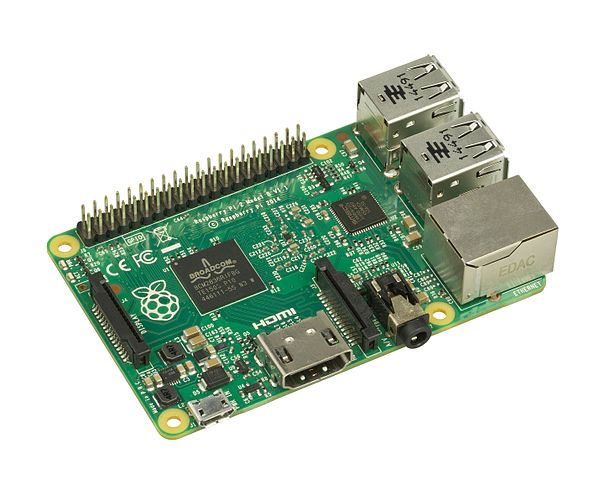
\includegraphics{Raspberry-Pi-2-Bare.jpg}
    \caption{M\'odulo Raspberry Pi 2B+}
    \label{fig:rpi2}
\end{figure}

\subsection{rpi2}

No es el prop\'osito de este trabajo ahondar sobre las caracter\'isticas de una rpi2, bastar\'a una breve descripci\'on de las capacidades que nos interesa.\\

Una rpi2 es una computadora de bajo costo del tama\~no de una tarjeta de cr\'edito. Existen diferentes modelos, para este proyecto necesitamos el que tiene un puerto ethernet y al menos un puerto USB. El sistema operativo corre desde una tarjeta microSD\footnote{Con una capacidad de \SI{4}{GB} estamos cubiertos.}.\\

A continuaci\'on una breve enumeraci\'on de las caracter\'isticas t\'ecnicas:

\begin{description}
    \item [CPU] \SI{900}{MHz} quad-core ARM Cortex-A7
    \item [RAM] \SI{1}{GB}
    \item [USB] $4$ puertos
    \item [ethernet] $1$ puerto de \SI{100}{MB}
    \item [Video] puerto HDMI
    \item [Audio] jack stereo de \SI{3,5}{mm}
    \item [interface] una para la c\'amara y otra para un display, adem\'as de un pinout GPIO.
\end{description}

\subsection{Raspbian}

Si decimos que una rpi2 es una \emph{computadora} podemos suponer que necesita un sistema operativo\footnote{Y hacemos bien en sospechar que se trata de una distribuci\'on GNU/Linux.}. En la p\'agina oficial de Raspberry Pi se encuentran disponibles varias alternativas, la que nos interesa es \emph{Raspbian}.\\

Raspbian es el sistema operativo oficial de la Fundaci\'on Raspberry Pi. Es un sistema operativo basado en \emph{Debian} y compilado para correr en una rpi2\footnote{El SO es tan completo y al mismo tiempo tan liviano que existe una versi\'on para PC, \emph{Raspbian Pi Desktop}.}.\\

Al momento de escribir este informe la \'ultima versi\'on disponible es de finales de junio de 2018, la versi\'on del kernel es 4.14. La \emph{versi\'on} de Raspian es \emph{Stretch}\footnote{En opini\'on del que escribe, el planeta Raspberry pertenece al universo Debian.}. Si bien la opci\'on popular es Raspbian con entorno gr\'afico vamos a optar por la versi\'on \emph{Lite}\footnote{No es otra cosa que el sistema base, lo que en la jerga se conoce como \emph{un debian pelado}.} (Figura~\ref{fig:raspbian}).\\

\begin{figure}
\centering
    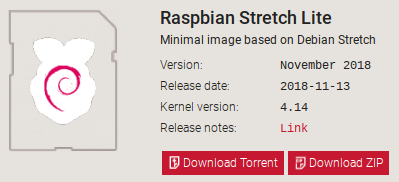
\includegraphics[scale=0.5]{pictos/raspbian-lite.png}
    \caption{Raspbian Lite}
    \label{fig:raspbian}
\end{figure}

La \emph{instalaci\'on} se trata de \emph{copiar} el sistema Raspbian en la tarjeta microSD. As\'i expresado es una sobresimplificaci\'on del procedimiento y un error de conceptos; pero bien pensado \emph{todo} en un sistema GNU/Linux es un \emph{archivo}; y a diferencia de una PC, donde encontramos distintos dispositivos con diferentes \emph{firmwares}\footnote{En el universo Windows se los conoce como \emph{drives}.} una rpi2 es id\'entica a otra rpi2 que podemos conseguir en un local de Bangladesh, por lo que s\'olo se necesita compilar el sistema operativo una vez, crear la imagen y hacerla accesible para cualquiera que necesite clonarla.\\

En el siguiente c\'odigo vemos c\'omo listamos los dispositivos conectados buscando la microSD, desmontamos y clonamos el sistema operativo\footnote{Algunos comandos necesitan derechos de \emph{root}.}. La imagen que provee el sitio ofical est\'a comprimida en un archivo \emph{zip} que se descarg\'o en el directorio \emph{/tmp} y se la descomprimi\'o ah\'i\footnote{Bajo \emph{systemd} el directorio /tmp es montado autom\'aticamente con un sistema de archivo \emph{tmpfs}, esto es, en la memoria RAM del sistema.}.

\begin{lstlisting}
!\#! blkid -o list
!\#! umount /media/pi/0403-0201
!\#! 7z x /tmp/2018-06-27-raspbian-stretch-lite.zip
!\#! dd bs=4M if=/tmp/2018-06-27-raspbian-stretch-lite.img of=/dev/mmcblk0 status=progress
\end{lstlisting}

\subsection{Energ\'ia}

Este proyecto necesita una fuente de alimentaci\'on que resuelva el problema de los cortes espor\'adicos de energ\'ia. Podr\'ia emplearse una UPS\footnote{\emph{Uninterruptible Power Supply.}} pero con un cargador de celular que disponga de al menos una salida de energ\'ia \emph{mientras se est\'a cargando} resuelve el problema.\\

No ahondaremos aqu\'i sobre los detalles del \emph{power bank}, el \'unico dato importante es la potencia que debe poder entregar en el momento de m\'aximo consumo, que es cuando la rpi2 bootea y cuando graba una fotograf\'ia en el USB (Cuadro~\ref{tab:energia}).

\begin{table}[h!]
    \begin{center}
        \begin{tabular}{lll}
        \cline{1-2}
        \multicolumn{1}{|l|}{\cellcolor[HTML]{EFEFEF}Situaci\'on}   & \multicolumn{1}{r|}{\cellcolor[HTML]{EFEFEF}Corriente}    & \\
        \cline{1-2}
        \multicolumn{1}{|l|}{boot + USB}                            & \multicolumn{1}{r|}{900-1400 mAh}                         & \\
        \cline{1-2}
        \multicolumn{1}{|l|}{ocioso (\emph{idle}) + USB}            & \multicolumn{1}{r|}{960 mAh}                              & \\
        \cline{1-2}
        \multicolumn{1}{|l|}{CPU con una carga al 400\% + USB}      & \multicolumn{1}{r|}{1250 mAh}                             & \\
        \cline{1-2}
        \multicolumn{1}{|l|}{idle + c\'amara + USB}                 & \multicolumn{1}{r|}{1200 mAh}                             &
        \end{tabular}
    \end{center}
    \caption{Consumo aproximado}
    \label{tab:energia}
\end{table}

\subsection{C\'amara}

Los creadores de rpi2 dispusieron de una interfase exclusiva para una c\'amara modular, que se conecta mediante un cable plano dise\~nado para romperse con facilidad (Figura~\ref{fig:ribbon}). Se compra, se conecta y funciona luego de habilitar el puerto. Consume alrededor de \SI{250}{mAh} desde el momento en que es habilitada (para el caso, desde el booteo); \'este es un factor a tener en cuenta porque suele creerse que s\'olo consume energ\'ia cuando captura una imagen o graba un video, lo cierto es que hay un leve aumento de consumo pero es el proceso de \emph{grabar} la imagen en el disco (la memoria USB en este caso).

\begin{figure}
\centering
    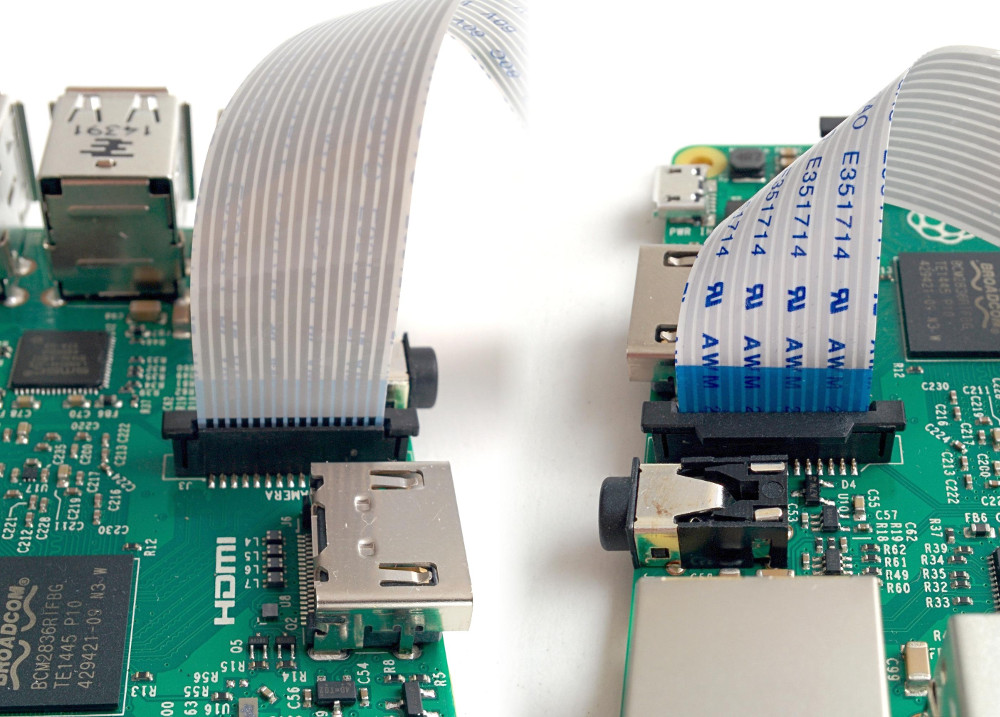
\includegraphics[scale=0.15]{connect-camera.jpg}
    \caption{Conexi\'on de la c\'amara modular}
    \label{fig:ribbon}
\end{figure}

\subsection{Memoria USB}

Tomando en cuenta que se van a capturar fotograf\'ias una vez por hora durante 14 d\'ias se obtiene el n\'umero de im\'agenes que se deben guardar en la memoria USB: $336$. Cada fotograf\'ia tiene una resoluci\'on de \SI{1280x720}{pixels}, cada p\'ixel necesita \SI{3}{B}\footnote{Uno por cada color \emph{RGB}.}, luego cada im\'agen es un archivo de \SI{2764800}{B}.\\

Dicho lo cual, necesitamos una memoria USB de \SI{1}{GB}\footnote{Exactamente \SI{928972800}{B}.}. Hace a\~nos que no se fabrican memorias USB de menos de \SI{4}{GB}; incluso se podr\'ia prescindir de la memoria USB porque el espacio que todav\'ia queda en la memoria mSD es m\'as que suficiente.

\subsubsection{3-2-1 backup rule}

Si no se ha cultivado un esp\'iritu aventurero es conveniente tener un \emph{backup}. Seguiremos la conocida regla \textbf{3-2-1} para pol\'iticas de backup (Figura~\ref{fig:321bkp}):
\begin{description}
    \item [3] copias de las im\'agenes
    \item [2] copias en medios f\'isicos distintos
    \item [1] copia fuera del lugar f\'isico
\end{description}

Resumiendo, una vez obtenida la imagen se guarda en un directorio de la tarjeta mSD, se hace una copia en la memoria USB y cada \SI{6}{h} se la sube a una carpeta alojada en un servicio cloud.

\begin{figure}
\centering
    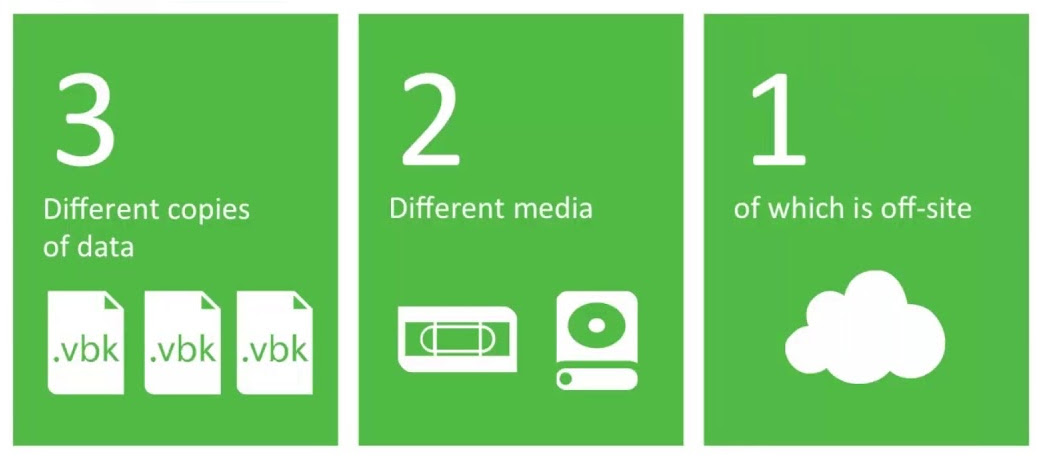
\includegraphics[scale=0.2]{321backup.jpg}
    \caption{3-2-1 backup rule}
    \label{fig:321bkp}
\end{figure}

\subsubsection{Automontaje}

En caso de una grave falla de energ\'ia, al punto de agotar la bater\'ia del power-bank, el sistema va a reiniciar en cuanto la energ\'ia se reestablezca. Se necesita, entonces, automontar la memoria USB. Systemd mediante, esta tarea es crear un archivo \emph{unit} del tipo \emph{mount} en el directorio \texttt{/etc/systemd/system}. Es necesario nombrar esta unit de acuerdo al punto de montaje, en este caso, \texttt{mnt-bkpUSB.mount}.

\begin{lstlisting}
!\#! mkdir /mnt/bkpUSB
!\#! touch /etc/systemd/system/mnt-bkpUSB.mount
\end{lstlisting}

Se busca el UUID\footnote{\emph{Universally Unique IDentifiers}, es una forma un\'ivoca de identificar un dispositivo de almacenamiento.} de la memoria USB:\\
\lstinline{# blkid}\\

Para finalmente editar la unidad de montaje como a continuaci\'on:

\begin{scriptsize}
%\begin{mdframed}
\begin{unitFrame}[/etc/systemd/system/mnt-bkpUSB.mount]
\begin{verbatim}
[Unit]
Description=USB backup
Before=local-fs.target umount.target

[Mount]
What=/dev/disk/by-uuid/87dcbe0c-1e1f-4de7-8f1e-65bcb37a4152
Where=/mnt/bkpUSB
Type=ext4
Options=defaults

[Install]
WantedBy=local-fs.target
\end{verbatim}
\end{unitFrame}
%\end{mdframed}
\end{scriptsize}

Veamos brevemente qu\'e es lo que configuramos en esta \emph{unidad}:

\begin{description}
\label{sec:wantedBy}
    \item [Description=] Aqu\'i debe indicarse brevemente y lo m\'as claro que se pueda qu\'e es lo que hace esta unidad.
    \item [Before=] En este caso le estamos indicando a systemd que retrase el inicio de local-fs.target y umount.target hasta que nuestra unidad termine de iniciar. Evitamos as\'i alg\'un conflicto (por ejemplo, que nuestra memoria USB se monte en /media/pi/ y no en /mnt/bkpUSB).\\
    \item [What=] Indicamos unequ\'ivocamente el dispositivo que queremos montar.
    \item [Where=] Indicamos d\'onde queremos montar ese dispositivo.
    \item [Type=] Cu\'al es el sistema de archivos que va a montar (\emph{filesystem}).
    \item [Options=] Las opciones de montaje, que conviene en \'este caso dejarlas predeterminadas.
    \item [WantedBy=] Aqu\'i indicamos qu\'e unidad o servicio va a iniciar a \'esta unidad. No lo maneja systemd directamente, sino cuando se lo instala (cosa que debemos hacer para completar el automontaje, esto es: \lstinline{# systemctl enable mnt-bkpUSB.mount}) se crea un enlace simb\'olico de esta unidad en el directorio \emph{local-fs.target.wants}, que cuando inicia local-fs.target inicia mnt-bkpUSB.mount\footnote{Momento, ?`no le indicamos en \texttt{Before=} que retrase el inicio de local-fs.target?, ?`por qu\'e le decimos ahora que sea local-fs.target quien inicie a mnt-bkpUSB.mount? Brevemente: systemd sabe que tiene que iniciar local-fs.target, no mnt-bkpUSB.mount, a resultas nuestra unidad de automontaje inicia \emph{antes} pero \emph{a pedido} de local-fs.target.}.
\end{description}

Con SysVinit hab\'ia que modificar el archivo \texttt{/etc/fstab} y agregar una l\'inea como la siguiente\footnote{La opci\'on \emph{auto} indica que se automonte.}:

\begin{scriptsize}
\begin{mdframed}
\begin{verbatim}
<file system>       <mount point>   <type>  <options>               <dump>  <pass>
UUID=87dcbe0c-1e1f-4d... /mnt/bkpUSB     ext4    defaults,noatime,auto   0       0
\end{verbatim}
\end{mdframed}
\end{scriptsize}

\subsubsection{Journaling}

No es imprescindible que la memoria USB tenga un sistema de archivos con \emph{journaling}. El journaling es una t\'ecnica implementada en algunos \emph{filesystems} que aseguran la integridad de los archivos; nos permite un alto grado de confianza cuando copiamos archivos de un medio a otro.\\

En los sistemas GNU/Linux es posible elegir entre varios filesystems, donde \textbf{ext4} es el favorito de muchas distribuciones. A efectos de ser prolijos, formateamos la memoria USB con \'ese filesystem\footnote{?`Por qu\'e no ntfs? Porque este informe puede prescindir de \emph{Windows}.}. Desmontamos la memoria USB\footnote{En una rpi2 el primer pendrive es asignado como /dev/sda.} y lo formateamos con una peligrosa facilidad:

\begin{lstlisting}
!\#! umount /dev/sda1
!\#! mkfs.ext4 /dev/sda1
\end{lstlisting}

\section{Servicios}

Los servicios ser\'an expuestos s\'olo en su objetivo, no describiremos el c\'odigo por muy simple que sea. Por ejemplo, vamos a suponer que para tomar una fotograf\'ia s\'olo debe ejecutarse un script al que llamaremos \emph{tomarFoto.sh}\footnote{El script puede estar en cualquier lugar, s\'olo debemos recordar asignarle el permiso de ejecuci\'on.}; para sincronizar\footnote{Sincronizar no es \emph{copiar}, es comparar la carpeta de origen con la de destino y dejarla igual, borrando los archivos que ya no est\'an en la carpeta origen y copiando los que todav\'ia no.} la carpeta de fotograf\'ias en la rpi2 con la carpeta alojada en el servidor \emph{Drive} no necesitamos un script porque se hace con una l\'inea de comando\footnote{Vamos a ignorar el control de errores, porque en alg\'un momento este informe tiene que terminarse.} por lo que la estructura es la misma.\\

Ha llegado el momento de configurar los servicios en systemd. Para entender cabalmente los servicios que se necesitan repasemos los requerimientos.\\

Por cada hora se toma una fotograf\'ia que es guardada en un directorio del sistema, /home/pi/Fotos, y se escribe una entrada registrando el evento. Entonces necesitamos una \emph{unit.timer}: \textbf{tomarFoto.timer}, que active una \emph{unit.service}: \textbf{tomarFoto.service}, que tome la fotograf\'ia y active otra \emph{unit.service}: \textbf{tomarFotoLog.service}, que realice el log. Cada vez que el directorio /home/pi/Fotos cambie (es decir, cuando se crea un nuevo archivo en \'el) se activa una \emph{unit.path}: \textbf{syncUSB.path}, que activa una \emph{unit.service}: \textbf{syncUSB.service} que sincroniza ese directorio con otro directorio en la memoria USB, que a su vez activa una \emph{unit.service}: \textbf{syncUSBLog.service}, que hace un logging\footnote{Acci\'on de realizar un log} de esta acci\'on (Figura~\ref{fig:tomarFoto}).

\begin{figure}[h!]
\centering
    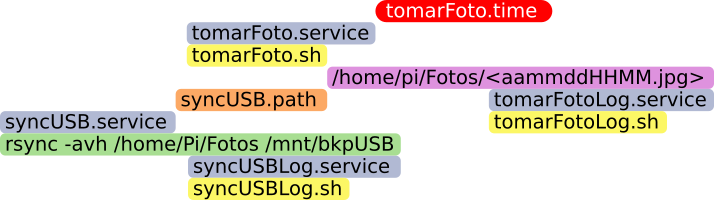
\includegraphics[scale=0.25]{pictos/tomarFoto.png}
    \caption{Algoritmo para tomar una foto}
    \label{fig:tomarFoto}
\end{figure}

Cada \SI{6}{h} se sincroniza la carpeta /home/pi/Fotos con una carpeta en el cloud de Drive y se hace un logging de esta acci\'on. Ya deber\'iamos sospechar lo que necesitamos, una \emph{unit.timer}: \textbf{syncDrive.timer}, que active una \emph{unit.service}: \textbf{syncDrive.service}, que sincronice y que a su vez active una \emph{unit.service}: \textbf{syncDriveLog.service}, que haga el log (Figura~\ref{fig:syncDrive}).

\begin{figure}[h!]
\centering
    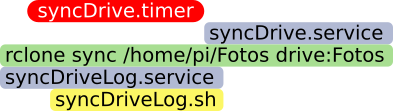
\includegraphics[scale=0.25]{pictos/syncDriver.png}
    \caption{Algoritmo para tomar sincronizar en la nube}
    \label{fig:syncDrive}
\end{figure}

Empecemos por el servicio que justifica este informe: \emph{tomarFoto.service}

\subsection{tomarFoto.service}

\begin{lstlisting}
!\#! touch /etc/systemd/system/tomarFoto.service
!\#! chmod 644 /etc/systemd/system/tomarFoto.service!\footnote{Por convenci\'on todos los usuarios tienen permiso de lectura y negados para la ejecuci\'on; y s\'olo el root deber\'ia poder editarlos.}!
!\#! vim /etc/systemd/system/tomarFoto.service
\end{lstlisting}

\begin{scriptsize}
\begin{unitFrame}[/etc/systemd/system/tomarForo.service]
\begin{verbatim}
[Unit]
Description=Captura una foto

[Service]
Type=oneshot
ExecStart=/home/pi/scripts/tomarFoto.sh
\end{verbatim}
\end{unitFrame}
\end{scriptsize}

Por convenci\'on las unit de servicio se nombran como el servicio que ejecutan.

\subsubsection{?`Unit?}

--\emph{Entiendo} ---dice un probable lector---, \emph{?`pero qu\'e es una \emph{unit}?}\\

En el supuesto improbable de que \'ese lector se est\'e anoticiando con \'este informe de systemd, a continuaci\'on una breve descripci\'on. Systemd es el administrador de servicios\footnote{Demonios.} que reemplaza al venerable SysVinit con un enfoque diferente del manejo de recursos, tanto dispositivos, puntos de montaje, sockets, etc. Por ejemplo, el tiempo de booteo se acorta \emph{dram\'aticamente} debido a que systemd implementa una agresiva paralelizaci\'on de los servicios, en contraste con SysVinit que es secuencial. Los scripts y daemons de SysVinit son compatibles con systemd.\\

Una de las ventajas de systemd es su simpleza en la configuraci\'on. La columna vertebral de systemd son las unit: archivos de texto plano que habitan en /lib/systemd/system con una extensi\'on que indica qu\'e tipo de unit es (service, path, mount point, target, timer, device, socket, etc.). Brevemente, una unit describe un recurso y le indica a systemd c\'omo debe activarlo. No todas las unit est\'an activadas al inicio, muchas inician s\'olo cuando son necesarias, optimizando el sistema de manera notable. Cuando una de \'estas units est\'a activa un link simb\'olico se crea en /etc/systemd/system. En este caso de estudio, vamos a crear las unit que se necesitan en este \'ultimo directorio, porque por convenci\'on s\'olo las unit \emph{nativas} del sistema operativo deben estar en /lib/systemd/system.\\

Retomando, la unit tomarFoto.service tiene dos secciones: \emph{[Unit]} y \emph{[Service]}. La primera es opcional (aunque rara vez se omite) y posee informaci\'on de la unit; es com\'un a todas. La otra secci\'on es espec\'ifica de este tipo de unit. 

\begin{description}
    \item [Description=] Esta secci\'on es descriptiva, pensada para la interfase del usuario.
    \item [Type=] Indica c\'omo debe activarse este servicio, \emph{qu\'e tipo de servicio es}. No nos interesa que systemd siga a este servicio luego de ejecutarse, por eso en lugar de \emph{simple} le indicamos \emph{oneshot}.
    \item [ExecStart=] Comandos con sus argumentos que ser\'an ejecutados cuando este servicio inicie. Sin embargo, como le indicamos que el Type es oneshot s\'olo hay que poner uno, que en este caso es tomarFoto.sh que est\'a alojado en el directorio /home/pi/scripts.
\end{description}

Ahora podemos tomar una foto de dos formas\footnote{en el supuesto que el script tomarFoto.sh cumpla lo que promete.}:

\begin{lstlisting}
!\$! /home/pi/scripts/tomarFoto.sh
\end{lstlisting}

o a trav\'es de systemd:

\begin{lstlisting}
!\$! systemctl start tomarFoto.service
\end{lstlisting}

\subsection{tomarFoto.path}

Analicemos la Figura~\ref{fig:tomarFoto}, al crear un archivo (la foto) en el directorio /home/pi/Fotos se dispara la unit syncUSB.service, ?`por qu\'e? Por la unit \emph{syncUSB.path}, que le indica a systemd que monitoree ese directorio; y cuando se produce un cambio systemd activa la unit asociada a syncUSB.path: \emph{syncUSB.service}.\\

Entonces, una vez creadas las unit como se hizo con tomarFoto.service procedemos a editarlas:

\begin{scriptsize}
\begin{unitFrame}[/etc/systemd/system/syncUSB.path]
\begin{verbatim}
[Unit]
Description=Monitorea el directorio Fotos

[Path]
PathModified=/home/pi/Fotos
\end{verbatim}
\end{unitFrame}
\end{scriptsize}

Este tipo de unit debe contener una secci\'on \emph{[Path]}

\begin{description}
    \item [PathModified=] Ruta absoluta del directorio o archivo a monitorear.
\end{description}

\subsection{rsync y rclone}

En la Figura~\ref{fig:tomarFoto} y Figura~\ref{fig:syncDrive} vemos que los servicios syncUSB.service y syncDrive.service no tienen un script bash correspondiente.

\begin{scriptsize}
\begin{unitFrame}[/etc/systemd/system/syncUSB.service]
\begin{verbatim}
[Unit]
Description=Sincroniza Fotos con el USB

[Service]
Type=oneshot
ExecStart=rsync -avh /home/pi/Fotos/ /mnt/bkpUSB/
\end{verbatim}
\end{unitFrame}
\end{scriptsize}

\begin{scriptsize}
\begin{unitFrame}[/etc/systemd/system/syncDrive.service]
\begin{verbatim}
[Unit]
Description=Sincroniza Fotos con el servicio Drive de Google

[Service]
Type=oneshot
ExecStart=rclone sync /home/pi/Fotos/ drive:Fotos
\end{verbatim}
\end{unitFrame}
\end{scriptsize}

En estos casos es innecesario crear sendos scripts, pues tendr\'ian la misma l\'inea de c\'odigo. Los programas \emph{rsync} y \emph{rclone} pueden instalarse directamente desde el repositorio de Debian:

\begin{lstlisting}
!\#! aptitude update && aptitude install -y rsync rclone
\end{lstlisting}

\'Esto es, utilizamos el gestor de paquetes \emph{aptitude}\footnote{Se dice que es un poco m\'as expeditivo y eficiente que apt (o apt-get).} para actualizar la base del repositorio y a continuaci\'on\footnote{Esa continuaci\'on est\'a indicada por los dos signos ampersand (\&\&).} instalamos rsync y rclone.\\

La estructura de rsync y rclone es cl\'asica: \emph{comando} \emph{opciones} \emph{origen} \emph{destino}

\subsection{tomarFotoLog.service}

A los efectos de ilustrar la activaci\'on de un servicio a pedido de otro es que en este informe se utiliza una unit para realizar el log del servicio realizado; de otro modo bien podr\'ia realizar esta tarea el mismo script que realiza la tarea (tomarFoto, syncUSB y syncDrive).\\

Entonces, creado como antes se procede a editar tomarFotoLog.service:

\begin{scriptsize}
\begin{unitFrame}[/etc/systemd/system/tomarFotoLog.service]
\begin{verbatim}
[Unit]
Description=Log de tomarFoto

[Service]
Type=oneshot
ExecStart=/home/pi/scripts/tomarFotoLog.sh

[Install]
WantedBy=tomarFoto.service
\end{verbatim}
\end{unitFrame}
\end{scriptsize}

Esta unit tiene una secci\'on \emph{[Install]} que las otras no necesitaban. Aqu\'i encontramos la informaci\'on que systemctl necesita para \emph{instalar} este servicio (ver Secci\'on~\ref{sec:wantedBy}).

\begin{description}
    \item [WantedBy=] Se le indica a systemctl que en la instalaci\'on de este servicio cree un enlace simb\'olico a esta unit dentro de la carpeta /etc/systemd/system/tomarFoto.service.wants (que ser\'a creada autom\'aticamente), de modo tal que cuando tomarFoto.service inicie tambi\'en lo haga tomarFotoLog.service.
\end{description}

Lo mismo se aplica para los servicios syncUSBLog.service y syncDriveLog.service:

\begin{scriptsize}
\begin{unitFrame}[/etc/systemd/system/syncUSBLog.service]
\begin{verbatim}
[Unit]
Description=Log de sincronizar con el USB

[Service]
Type=oneshot
ExecStart=/home/pi/scripts/syncUSBLog.sh

[Install]
WantedBy=syncUSB.service
\end{verbatim}
\end{unitFrame}
\end{scriptsize}

\begin{scriptsize}
\begin{unitFrame}[/etc/systemd/system/syncDriveLog.service]
\begin{verbatim}
[Unit]
Description=Log de sincronizar con Drive

[Service]
Type=oneshot
ExecStart=/home/pi/scripts/syncDriveLog.sh

[Install]
WantedBy=syncDrive.service
\end{verbatim}
\end{unitFrame}
\end{scriptsize}

\section{Timers}

Hasta ahora s\'olo se han configurado los servicios que se ejecutan a pedido del usuario. Seg\'un las especificaciones el sistema tiene que ser completamente autom\'atico. En primera instancia podr\'iamos configurar los servicios \emph{cron} mediante\footnote{A partir de systemd, cron es un servicio de systemd.}, pero systemd cuenta con la herramienta adecuada: las unit \emph{timer}.\\

Una unit con la extensi\'on \emph{timer} contiene la informaci\'on necesaria para que systemd active los servicios que deben ser activados por tiempo.\\

Entonces, cada \SI{60}{min} se ejecutan tres acciones (que ya est\'an configuradas):

\begin{enumerate}
    \item tomar foto
    \item sincronizar carpeta de fotos de la rpi2 con la memoria USB
    \item log
\end{enumerate}

Y cada \SI{6}{h} se ejecutan dos scripts:

\begin{enumerate}
    \item sincronizar carpeta de fotos de la rpi2 con el servidor Drive
    \item log
\end{enumerate}

Los servicios son disparados por \emph{systemd} y deben ser nombrados en correspondencia con la unit.service que disparan. Deben contener una secci\'on \emph{[Timer]} con las instrucciones de cu\'ando o cada cu\'anto debe activarse. Entonces:

\begin{scriptsize}
\begin{unitFrame}[/etc/systemd/system/tomarFoto.timer]
\begin{verbatim}
[Unit]
Description=Temporizador de tomarFoto

[Timer]
OnCalendar=hourly

[Install]
WantedBy=timers.target
\end{verbatim}
\end{unitFrame}
\end{scriptsize}

\begin{description}
    \item [OnCalendar=] Define un horario en tiempo real (esto es, la hora del reloj de pared). En el caso de tomarFoto, \emph{hourly} es una abreviaci\'on que entiende systemd (una vez cada hora, a partir de las 00:00 a.m.).
\end{description}

\begin{scriptsize}
\begin{unitFrame}[/etc/systemd/system/syncDrive.timer]
\begin{verbatim}
[Unit]
Description=Temporizador de syncDrive

[Timer]
OnCalendar=00:30/6
# cada 6 horas a partir de las 00:30 a.m.

[Install]
WantedBy=timers.target
\end{verbatim}
\end{unitFrame}
\end{scriptsize}

Subidos en el tren de la did\'actica configuramos el inicio de syncDrive de forma tal que no coincida con syncUSB: le indicamos a systemd que el servicio syncDrive debe repetirse cada 6 horas a partir de la 00:30 a.m.\footnote{Invito a los usuarios veteranos de GNU/Linux a configurar cron con \'estas mismas especificaciones.}. Una manera m\'as simple hubiera sido:

\begin{lstlisting}
OnCalendar=6h
\end{lstlisting}

Por \'ultimo, deben activarse las unit.timer:

\begin{lstlisting}
!\#! systemctl enable tomarFoto.timer
!\#! systemctl enable syncDrive.timer
\end{lstlisting}

\section{Conclusi\'on}

Este informe (disfrazado de \emph{howto}) no pretende hacer una valoraci\'on entre sysvninit y systemd, sino de proporcionar una gu\'ia para quienes necesiten resolver problemas como el planteado (completamente ficticio) y no quieran fatigar p\'aginas y p\'aginas de internet que todav\'ia est\'an analizando si systemd deber\'ia haber reemplazado a sysvinit; o leyendo una y otra vez los principales comandos de systemd (start, status, stop, etc) y c\'omo se relacionan con los de sysvinit.\\

La mayor cr\'itica (y probablemente cierta) es que systemd parece ir en contra de la filosofia de unix: evitar los programas monoliticos (un programa por cada tarea).\\

Sin embargo Debian ha decidido (desde \emph{Jessie}) que su versi\'on estable inicia con systemd. De todos los argumentos a favor creo que es el m\'as breve y determinante.\\

Devuan es una distribuci\'on \emph{fork} de Debian, pero todav\'ia tiene como PID 1 a init. Es decir, es Debian sin systemd. ?`Hasta cu\'ando? Nadie lo puede asegurar, ya que las principales distros han optado por systemd.\\

En su obligado libro \emph{En El Principio Fu\'e La L\'inea De Comandos}, Neal Stephenson parece reflexionar (all\'a por 1999) sobre sysvinit: \emph{[...] Linux trata con el problema del cruft\footnote{En la jerga significa algo fuera de uso, desactualizado. Aqu\'i el autor hace referencia al problema de mantener retrocompatibilidad en las nuevas versiones de un sistema operativo con las anteriores.} del mismo modo en que los esquimales trataban con sus jubilados: si insistes en usar viejas versiones de software Linux, antes o después acabarás por encontrarte flotando por el Estrecho de Bering en un iceberg cada vez más pequeño.}

\section{Bibliograf\'ia}

Gran parte de este informe est\'a documentado en base a los manuales del sistema (Figura~\ref{fig:rtfm}).\\

As\'i por ejemplo, para saber acerca de las unit en systemd basta con tipear desde la terminal:

\begin{lstlisting}
!\$! man systemd.unit 
\end{lstlisting}

O en el caso de las unit timer:

\begin{lstlisting}
!\$! man systemd.timer 
\end{lstlisting}

La verdad es que los art\'iculos web que consult\'e a lo largo de este informe siempre fueron la punta del iceberg de alg\'un manual del sistema.

\begin{figure}
\centering
    
\includegraphics[scale=0.25]{Mao_RTFM.png}
    \caption{RTFM}
    \label{fig:rtfm}
\end{figure}

\subsection{algunos art\'iculos web consultados}

\begin{scriptsize}
\begin{verbatim}
https://opensource.com/resources/raspberry-pi
https://www.raspberrypi.org/help/what-%20is-a-raspberry-pi/
https://www.pidramble.com/wiki/benchmarks/power-consumption
https://wiki.archlinux.org/index.php/tmpfs
https://picamera.readthedocs.io/en/latest/fov.html
https://www.veeam.com/blog/how-to-follow-the-3-2-1-backup-rule-with-veeam-backup-replication.html
\end{verbatim}
\end{scriptsize}

\subsubsection{raspbian boot}

\begin{scriptsize}
\begin{verbatim}
https://raspberrypi.stackexchange.com/questions/39959/raspbian-boot-process-and-the-partition-table
\end{verbatim}
\end{scriptsize}

\subsubsection{journal checksumming}

\begin{scriptsize}
\begin{verbatim}
https://www.kernel.org/doc/Documentation/filesystems/ext4.txt
https://ext4.wiki.kernel.org/index.php/Ext4_Metadata_Checksums
\end{verbatim}
\end{scriptsize}

\subsubsection{systemd}

\begin{scriptsize}
\begin{verbatim}
https://www.suse.com/media/white-paper/systemd_in_suse_linux_enterprise_12_white_paper.pdf   

https://oguya.ch/posts/2015-09-01-systemd-mount-partition/
https://www.digitalocean.com/community/tutorials/understanding-systemd-units-and-unit-files
https://www.digitalocean.com/community/tutorials/how-to-use-systemctl-to-manage-systemd-services-and-units
https://www.shellhacks.com/systemd-service-file-example/
https://www.redpill-linpro.com/sysadvent/2016/12/07/systemd-timers.html
\end{verbatim}
\end{scriptsize}

\subsubsection{logging}

\begin{scriptsize}
\begin{verbatim}
https://serverfault.com/questions/573946/how-can-i-send-a-message-to-the-systemd-journal-from-the-command-line
https://www.loggly.com/ultimate-guide/linux-logging-with-systemd/
\end{verbatim}
\end{scriptsize}

\subsubsection{gnu/linux philosophy}

\begin{scriptsize}
\begin{verbatim}
https://www.tldp.org/LDP/GNU-Linux-Tools-Summary/html/c1089.htm
\end{verbatim}
\end{scriptsize}

\subsubsection{im\'agenes ilustrativas}

\begin{scriptsize}
\begin{verbatim}
https://en.wikipedia.org/wiki/Raspberry_Pi#/media/File:Raspberry-Pi-2-Bare-BR.jpg
https://projects.raspberrypi.org/en/projects/getting-started-with-picamera/6
https://www.raspberrypi.org/documentation/usage/camera/raspicam/raspistill.md
https://knowyourmeme.com/photos/17668-rtfm
\end{verbatim}
\end{scriptsize}

\newpage
\section{GNU Free Documentation License}
\begin{scriptsize}
GNU Free Documentation License\\

Version 1.3, 3 November 2008\\

Copyright © 2000, 2001, 2002, 2007, 2008 Free Software Foundation, Inc. \texttt{https://fsf.org/}\\

Everyone is permitted to copy and distribute verbatim copies of this license document, but changing it is not allowed.\\


0. PREAMBLE
The purpose of this License is to make a manual, textbook, or other functional and useful document "free" in the sense of freedom: to assure everyone the effective freedom to copy and redistribute it, with or without modifying it, either commercially or noncommercially. Secondarily, this License preserves for the author and publisher a way to get credit for their work, while not being considered responsible for modifications made by others.

This License is a kind of "copyleft", which means that derivative works of the document must themselves be free in the same sense. It complements the GNU General Public License, which is a copyleft license designed for free software.

We have designed this License in order to use it for manuals for free software, because free software needs free documentation: a free program should come with manuals providing the same freedoms that the software does. But this License is not limited to software manuals; it can be used for any textual work, regardless of subject matter or whether it is published as a printed book. We recommend this License principally for works whose purpose is instruction or reference.\\

1. APPLICABILITY AND DEFINITIONS
This License applies to any manual or other work, in any medium, that contains a notice placed by the copyright holder saying it can be distributed under the terms of this License. Such a notice grants a world-wide, royalty-free license, unlimited in duration, to use that work under the conditions stated herein. The "Document", below, refers to any such manual or work. Any member of the public is a licensee, and is addressed as "you". You accept the license if you copy, modify or distribute the work in a way requiring permission under copyright law.

A "Modified Version" of the Document means any work containing the Document or a portion of it, either copied verbatim, or with modifications and/or translated into another language.

A "Secondary Section" is a named appendix or a front-matter section of the Document that deals exclusively with the relationship of the publishers or authors of the Document to the Document's overall subject (or to related matters) and contains nothing that could fall directly within that overall subject. (Thus, if the Document is in part a textbook of mathematics, a Secondary Section may not explain any mathematics.) The relationship could be a matter of historical connection with the subject or with related matters, or of legal, commercial, philosophical, ethical or political position regarding them.

The "Invariant Sections" are certain Secondary Sections whose titles are designated, as being those of Invariant Sections, in the notice that says that the Document is released under this License. If a section does not fit the above definition of Secondary then it is not allowed to be designated as Invariant. The Document may contain zero Invariant Sections. If the Document does not identify any Invariant Sections then there are none.

The "Cover Texts" are certain short passages of text that are listed, as Front-Cover Texts or Back-Cover Texts, in the notice that says that the Document is released under this License. A Front-Cover Text may be at most 5 words, and a Back-Cover Text may be at most 25 words.

A "Transparent" copy of the Document means a machine-readable copy, represented in a format whose specification is available to the general public, that is suitable for revising the document straightforwardly with generic text editors or (for images composed of pixels) generic paint programs or (for drawings) some widely available drawing editor, and that is suitable for input to text formatters or for automatic translation to a variety of formats suitable for input to text formatters. A copy made in an otherwise Transparent file format whose markup, or absence of markup, has been arranged to thwart or discourage subsequent modification by readers is not Transparent. An image format is not Transparent if used for any substantial amount of text. A copy that is not "Transparent" is called "Opaque".

Examples of suitable formats for Transparent copies include plain ASCII without markup, Texinfo input format, LaTeX input format, SGML or XML using a publicly available DTD, and standard-conforming simple HTML, PostScript or PDF designed for human modification. Examples of transparent image formats include PNG, XCF and JPG. Opaque formats include proprietary formats that can be read and edited only by proprietary word processors, SGML or XML for which the DTD and/or processing tools are not generally available, and the machine-generated HTML, PostScript or PDF produced by some word processors for output purposes only.

The "Title Page" means, for a printed book, the title page itself, plus such following pages as are needed to hold, legibly, the material this License requires to appear in the title page. For works in formats which do not have any title page as such, "Title Page" means the text near the most prominent appearance of the work's title, preceding the beginning of the body of the text.

The "publisher" means any person or entity that distributes copies of the Document to the public.

A section "Entitled XYZ" means a named subunit of the Document whose title either is precisely XYZ or contains XYZ in parentheses following text that translates XYZ in another language. (Here XYZ stands for a specific section name mentioned below, such as "Acknowledgements", "Dedications", "Endorsements", or "History".) To "Preserve the Title" of such a section when you modify the Document means that it remains a section "Entitled XYZ" according to this definition.

The Document may include Warranty Disclaimers next to the notice which states that this License applies to the Document. These Warranty Disclaimers are considered to be included by reference in this License, but only as regards disclaiming warranties: any other implication that these Warranty Disclaimers may have is void and has no effect on the meaning of this License.\\

2. VERBATIM COPYING
You may copy and distribute the Document in any medium, either commercially or noncommercially, provided that this License, the copyright notices, and the license notice saying this License applies to the Document are reproduced in all copies, and that you add no other conditions whatsoever to those of this License. You may not use technical measures to obstruct or control the reading or further copying of the copies you make or distribute. However, you may accept compensation in exchange for copies. If you distribute a large enough number of copies you must also follow the conditions in section 3.

You may also lend copies, under the same conditions stated above, and you may publicly display copies.\\

3. COPYING IN QUANTITY
If you publish printed copies (or copies in media that commonly have printed covers) of the Document, numbering more than 100, and the Document's license notice requires Cover Texts, you must enclose the copies in covers that carry, clearly and legibly, all these Cover Texts: Front-Cover Texts on the front cover, and Back-Cover Texts on the back cover. Both covers must also clearly and legibly identify you as the publisher of these copies. The front cover must present the full title with all words of the title equally prominent and visible. You may add other material on the covers in addition. Copying with changes limited to the covers, as long as they preserve the title of the Document and satisfy these conditions, can be treated as verbatim copying in other respects.

If the required texts for either cover are too voluminous to fit legibly, you should put the first ones listed (as many as fit reasonably) on the actual cover, and continue the rest onto adjacent pages.

If you publish or distribute Opaque copies of the Document numbering more than 100, you must either include a machine-readable Transparent copy along with each Opaque copy, or state in or with each Opaque copy a computer-network location from which the general network-using public has access to download using public-standard network protocols a complete Transparent copy of the Document, free of added material. If you use the latter option, you must take reasonably prudent steps, when you begin distribution of Opaque copies in quantity, to ensure that this Transparent copy will remain thus accessible at the stated location until at least one year after the last time you distribute an Opaque copy (directly or through your agents or retailers) of that edition to the public.

It is requested, but not required, that you contact the authors of the Document well before redistributing any large number of copies, to give them a chance to provide you with an updated version of the Document.\\

4. MODIFICATIONS
You may copy and distribute a Modified Version of the Document under the conditions of sections 2 and 3 above, provided that you release the Modified Version under precisely this License, with the Modified Version filling the role of the Document, thus licensing distribution and modification of the Modified Version to whoever possesses a copy of it. In addition, you must do these things in the Modified Version:

A. Use in the Title Page (and on the covers, if any) a title distinct from that of the Document, and from those of previous versions (which should, if there were any, be listed in the History section of the Document). You may use the same title as a previous version if the original publisher of that version gives permission.
B. List on the Title Page, as authors, one or more persons or entities responsible for authorship of the modifications in the Modified Version, together with at least five of the principal authors of the Document (all of its principal authors, if it has fewer than five), unless they release you from this requirement.
C. State on the Title page the name of the publisher of the Modified Version, as the publisher.
D. Preserve all the copyright notices of the Document.
E. Add an appropriate copyright notice for your modifications adjacent to the other copyright notices.
F. Include, immediately after the copyright notices, a license notice giving the public permission to use the Modified Version under the terms of this License, in the form shown in the Addendum below.
G. Preserve in that license notice the full lists of Invariant Sections and required Cover Texts given in the Document's license notice.
H. Include an unaltered copy of this License.
I. Preserve the section Entitled "History", Preserve its Title, and add to it an item stating at least the title, year, new authors, and publisher of the Modified Version as given on the Title Page. If there is no section Entitled "History" in the Document, create one stating the title, year, authors, and publisher of the Document as given on its Title Page, then add an item describing the Modified Version as stated in the previous sentence.
J. Preserve the network location, if any, given in the Document for public access to a Transparent copy of the Document, and likewise the network locations given in the Document for previous versions it was based on. These may be placed in the "History" section. You may omit a network location for a work that was published at least four years before the Document itself, or if the original publisher of the version it refers to gives permission.
K. For any section Entitled "Acknowledgements" or "Dedications", Preserve the Title of the section, and preserve in the section all the substance and tone of each of the contributor acknowledgements and/or dedications given therein.
L. Preserve all the Invariant Sections of the Document, unaltered in their text and in their titles. Section numbers or the equivalent are not considered part of the section titles.
M. Delete any section Entitled "Endorsements". Such a section may not be included in the Modified Version.
N. Do not retitle any existing section to be Entitled "Endorsements" or to conflict in title with any Invariant Section.
O. Preserve any Warranty Disclaimers.
If the Modified Version includes new front-matter sections or appendices that qualify as Secondary Sections and contain no material copied from the Document, you may at your option designate some or all of these sections as invariant. To do this, add their titles to the list of Invariant Sections in the Modified Version's license notice. These titles must be distinct from any other section titles.

You may add a section Entitled "Endorsements", provided it contains nothing but endorsements of your Modified Version by various parties—for example, statements of peer review or that the text has been approved by an organization as the authoritative definition of a standard.

You may add a passage of up to five words as a Front-Cover Text, and a passage of up to 25 words as a Back-Cover Text, to the end of the list of Cover Texts in the Modified Version. Only one passage of Front-Cover Text and one of Back-Cover Text may be added by (or through arrangements made by) any one entity. If the Document already includes a cover text for the same cover, previously added by you or by arrangement made by the same entity you are acting on behalf of, you may not add another; but you may replace the old one, on explicit permission from the previous publisher that added the old one.

The author(s) and publisher(s) of the Document do not by this License give permission to use their names for publicity for or to assert or imply endorsement of any Modified Version.\\

5. COMBINING DOCUMENTS
You may combine the Document with other documents released under this License, under the terms defined in section 4 above for modified versions, provided that you include in the combination all of the Invariant Sections of all of the original documents, unmodified, and list them all as Invariant Sections of your combined work in its license notice, and that you preserve all their Warranty Disclaimers.

The combined work need only contain one copy of this License, and multiple identical Invariant Sections may be replaced with a single copy. If there are multiple Invariant Sections with the same name but different contents, make the title of each such section unique by adding at the end of it, in parentheses, the name of the original author or publisher of that section if known, or else a unique number. Make the same adjustment to the section titles in the list of Invariant Sections in the license notice of the combined work.

In the combination, you must combine any sections Entitled "History" in the various original documents, forming one section Entitled "History"; likewise combine any sections Entitled "Acknowledgements", and any sections Entitled "Dedications". You must delete all sections Entitled "Endorsements".\\

6. COLLECTIONS OF DOCUMENTS
You may make a collection consisting of the Document and other documents released under this License, and replace the individual copies of this License in the various documents with a single copy that is included in the collection, provided that you follow the rules of this License for verbatim copying of each of the documents in all other respects.

You may extract a single document from such a collection, and distribute it individually under this License, provided you insert a copy of this License into the extracted document, and follow this License in all other respects regarding verbatim copying of that document.\\

7. AGGREGATION WITH INDEPENDENT WORKS
A compilation of the Document or its derivatives with other separate and independent documents or works, in or on a volume of a storage or distribution medium, is called an "aggregate" if the copyright resulting from the compilation is not used to limit the legal rights of the compilation's users beyond what the individual works permit. When the Document is included in an aggregate, this License does not apply to the other works in the aggregate which are not themselves derivative works of the Document.

If the Cover Text requirement of section 3 is applicable to these copies of the Document, then if the Document is less than one half of the entire aggregate, the Document's Cover Texts may be placed on covers that bracket the Document within the aggregate, or the electronic equivalent of covers if the Document is in electronic form. Otherwise they must appear on printed covers that bracket the whole aggregate.\\

8. TRANSLATION
Translation is considered a kind of modification, so you may distribute translations of the Document under the terms of section 4. Replacing Invariant Sections with translations requires special permission from their copyright holders, but you may include translations of some or all Invariant Sections in addition to the original versions of these Invariant Sections. You may include a translation of this License, and all the license notices in the Document, and any Warranty Disclaimers, provided that you also include the original English version of this License and the original versions of those notices and disclaimers. In case of a disagreement between the translation and the original version of this License or a notice or disclaimer, the original version will prevail.

If a section in the Document is Entitled "Acknowledgements", "Dedications", or "History", the requirement (section 4) to Preserve its Title (section 1) will typically require changing the actual title.\\

9. TERMINATION
You may not copy, modify, sublicense, or distribute the Document except as expressly provided under this License. Any attempt otherwise to copy, modify, sublicense, or distribute it is void, and will automatically terminate your rights under this License.

However, if you cease all violation of this License, then your license from a particular copyright holder is reinstated (a) provisionally, unless and until the copyright holder explicitly and finally terminates your license, and (b) permanently, if the copyright holder fails to notify you of the violation by some reasonable means prior to 60 days after the cessation.

Moreover, your license from a particular copyright holder is reinstated permanently if the copyright holder notifies you of the violation by some reasonable means, this is the first time you have received notice of violation of this License (for any work) from that copyright holder, and you cure the violation prior to 30 days after your receipt of the notice.

Termination of your rights under this section does not terminate the licenses of parties who have received copies or rights from you under this License. If your rights have been terminated and not permanently reinstated, receipt of a copy of some or all of the same material does not give you any rights to use it.\\

10. FUTURE REVISIONS OF THIS LICENSE
The Free Software Foundation may publish new, revised versions of the GNU Free Documentation License from time to time. Such new versions will be similar in spirit to the present version, but may differ in detail to address new problems or concerns. See https://www.gnu.org/licenses/.

Each version of the License is given a distinguishing version number. If the Document specifies that a particular numbered version of this License "or any later version" applies to it, you have the option of following the terms and conditions either of that specified version or of any later version that has been published (not as a draft) by the Free Software Foundation. If the Document does not specify a version number of this License, you may choose any version ever published (not as a draft) by the Free Software Foundation. If the Document specifies that a proxy can decide which future versions of this License can be used, that proxy's public statement of acceptance of a version permanently authorizes you to choose that version for the Document.\\

11. RELICENSING
"Massive Multiauthor Collaboration Site" (or "MMC Site") means any World Wide Web server that publishes copyrightable works and also provides prominent facilities for anybody to edit those works. A public wiki that anybody can edit is an example of such a server. A "Massive Multiauthor Collaboration" (or "MMC") contained in the site means any set of copyrightable works thus published on the MMC site.

"CC-BY-SA" means the Creative Commons Attribution-Share Alike 3.0 license published by Creative Commons Corporation, a not-for-profit corporation with a principal place of business in San Francisco, California, as well as future copyleft versions of that license published by that same organization.

"Incorporate" means to publish or republish a Document, in whole or in part, as part of another Document.

An MMC is "eligible for relicensing" if it is licensed under this License, and if all works that were first published under this License somewhere other than this MMC, and subsequently incorporated in whole or in part into the MMC, (1) had no cover texts or invariant sections, and (2) were thus incorporated prior to November 1, 2008.

The operator of an MMC Site may republish an MMC contained in the site under CC-BY-SA on the same site at any time before August 1, 2009, provided the MMC is eligible for relicensing.\\

ADDENDUM: How to use this License for your documents
To use this License in a document you have written, include a copy of the License in the document and put the following copyright and license notices just after the title page:

    Copyright (C)  YEAR  YOUR NAME.
    Permission is granted to copy, distribute and/or modify this document
    under the terms of the GNU Free Documentation License, Version 1.3
    or any later version published by the Free Software Foundation;
    with no Invariant Sections, no Front-Cover Texts, and no Back-Cover Texts.
    A copy of the license is included in the section entitled "GNU
    Free Documentation License".
If you have Invariant Sections, Front-Cover Texts and Back-Cover Texts, replace the "with … Texts." line with this:

    with the Invariant Sections being LIST THEIR TITLES, with the
    Front-Cover Texts being LIST, and with the Back-Cover Texts being LIST.
If you have Invariant Sections without Cover Texts, or some other combination of the three, merge those two alternatives to suit the situation.

If your document contains nontrivial examples of program code, we recommend releasing these examples in parallel under your choice of free software license, such as the GNU General Public License, to permit their use in free software.
\end{scriptsize}

\end{document}